\documentclass[10pt,twocolumn,letterpaper]{article}

\usepackage{cvpr}
\usepackage{times}
\usepackage{epsfig}
\usepackage{graphicx}
\usepackage{amsmath}
\usepackage{amssymb}
\usepackage{longtable}
\usepackage{tabularx,ragged2e}

\usepackage{subfig}
\usepackage{float}

% Include other packages here, before hyperref.

% If you comment hyperref and then uncomment it, you should delete
% egpaper.aux before re-running latex.  (Or just hit 'q' on the first latex
% run, let it finish, and you should be clear).
\usepackage[breaklinks=true,bookmarks=false]{hyperref}

\cvprfinalcopy % *** Uncomment this line for the final submission

\def\cvprPaperID{****} % *** Enter the CVPR Paper ID here
\def\httilde{\mbox{\tt\raisebox{-.5ex}{\symbol{126}}}}


% Pages are numbered in submission mode, and unnumbered in camera-ready
%\ifcvprfinal\pagestyle{empty}\fi
\setcounter{page}{1}
\begin{document}


%%%%%%%%% TITLE
\title{CIS520 Project: Hotel Cancellation Prediction}
\author{Yifei Li\\
School of Engineering and Applied Science\\
University of Pennsylvania\\
{\tt\small liyifei@seas.upenn.edu}
% For a paper whose authors are all at the same institution,
% omit the following lines up until the closing ``}''.
% Additional authors and addresses can be added with ``\and'',
% just like the second author.
% To save space, use either the email address or home page, not both
\and
Zhijian Yang\\
School of Engineering and Applied Science\\
University of Pennsylvania\\
{\tt\small zjyang@seas.upenn.edu}
}

\maketitle
%\thispagestyle{empty}

%%%%%%%%% ABSTRACT
\begin{abstract}
   The demand forecast is critical to the hospitality industry which always suffers from the market fluctuations. Compared to the traditional statistics and time series model used in hotel revenue management, the machine learning approaches have great potential to enhance the hotel demand prediction by analyzing the customer characteristics. We compared the performance of different machine learning models from classical techniques to deep learning architecture DeepFM, tuning out that a soft-voting estimator comprised of a tuned neural network, random forest and decision tree has an outstanding 97.52\% accuracy. Besides, the impact of dataset imbalance and hyperparameter tuning have been explored and discussed.
\end{abstract}


%%%%%%%%% CODE LINKS
{\small \textbf{Notebook links}: 
    (1) \href{https://github.com/realliyifei/ML-Project-Hotel-Cancellation-Prediction/blob/main/Data_Cleaning_and_Visualization.ipynb}
        {\emph{Dataset Cleaning and Visualization}} \\
    (2) \href{https://github.com/realliyifei/ML-Project-Hotel-Cancellation-Prediction/blob/main/Basic_Models_Experiment.ipynb}
        {\emph{Basic Models Experiment}}
    (3) \href{https://github.com/realliyifei/ML-Project-Hotel-Cancellation-Prediction/blob/main/Advanced_Models_Exploration.ipynb} 
        {\emph{Advanced Models Exploration}} }


%%%%%%%%% BODY TEXT
\section{Motivation}
In hospitality industry, the customer demands are seasonal and fluctuating for various reasons. The customer criteria such as travel frequency and service expectations plays a significant role in the hotel market. An accurate hotel demand prediction based on these customer features is valuable for revenue management by optimizing the room occupancy~\cite{weatherford2003comparison} while avoiding the risk of reputation damage caused by an excessive overbooking.

Machine learning models can seize both the breadth and depth of customer characteristics and have the potential to outperform the traditional hotel forecasting methods which are merely based on the date or several features. Besides, as a seasonal service industry, in hospitality, time-sensitive approaches such as classical time series model is meaningful to the demand prediction. Last, it's meaningful to see whether the model architectures from other fields such as recommendation system can be transferred to hotel demand prediction and work well.


%-------------------------------------------------------------------------
\section{Related Work}
The old school forecast models of hotel demand can be put in three categories: historical booking models, advanced booking models and combined models, involving deeply in time series and classical regression~\cite{weatherford2003comparison}.

As the emergence of machine learning, their applications in hotel industry rapidly grow up. Y. Zhang~\cite{ZhangApproaches} applies multiple classical machine learning models in hotel demand forecast based on pricing, location, etc., ending up that these approaches especially SVM and random forest beat the traditional model by empirical study. Also, S{\'a}nchez-Medina \etal~\cite{sanchez2020using} explores the usage of neural networks cooperated with genetic algorithms to predict not only the cancellation rate but also the likely customer who may cancel the room. Also, this techniques can set the structural parameters to find an optimal solution while lowing the risk of being stuck in the local maxima. The necessity of collecting the customer's historical records for hospitality enterprises as key asset has also been addressed from a managerial point of view.

Besides, there are increasing deep learning deployments in hotel demand forecast. B. Zhang \etal~\cite{zhang2019forecasting} explores the potential of LSTM model integrating the internet search index on the hotel accommodation demand forecast, showing the robustness of this model by large and different datasets. Compared to its benchmark models, the artical's novel constructed forecasting method can largely simulate the overnigt customer's dynamic features and hereby optimizes the prediction. Further, Q. Zhang \etal~\cite{Zhang2019Deep} introduces a deep learning based dynamic pricing model which contains DeepFM, seq2seq and DNN frameworks for hotel revenue management. It can improve the prediction accuracy without a very complex feature engineering.

Last, for the methods, Kumari and Srivastava~\cite{kumari2017machine} completed a taxonomy for binary classification. A bunch of machine learning approaches like SVM, decision tree, and nueral network are mentioned and compared, though there is not a model with absolute advantage since the standard and requirement changes as the dataset differs.



%-------------------------------------------------------------------------
\section{Dataset}

%-------------------------------------------------------------------------
\subsection{Introduction}
In this project we use a dataset\footnote{Source:  \url{https://ars.els-cdn.com/content/image/1-s2.0-S2352340918315191-mmc2.zip}} provided by Nuno Antonio. It contains hotel booking information between July 1st, 2015 and August 31st, 2017~\cite{ANTONIO201941}. There are in total 119,390 bookings data from a city hotel and a resort hotel, with 32 features. The features are a mixture of 15 categorical variables and 17 numerical variables (Table~\ref{tab:DataTypes}), ranging from hotel type and country location to canceled status and arrival time. 

\begin{table}[ht]
\begin{center}
\begin{tabular}{|c|c|c|} \hline
    Integer & \multicolumn{2}{p{6cm}|}{\RaggedRight \emph{LeadTime, ArrivalDateYear, ArrivalDateWeekNumber, ArrivalDateDayOfMonth, StaysInWeekendNights, StaysInWeekNights, Adults, Babies, IsRepeatedGuest, PreviousCancellations, PreviousBookingsNotCanceled, BookingChanges, DaysInWaitingList, RequiredCarParkingSpaces, TotalOfSpecialRequests}} \\ \hline
    Float &  \multicolumn{2}{p{6cm}|}{\RaggedRight \emph{Children, Agent, Company, ADR}} \\ \hline
    Object & \multicolumn{2}{p{6cm}|}{\RaggedRight \emph{ArrivalDateMonth, Meal, Country, MarketSegment, DistributionChannel, ReservedRoomType, AssignedRoomType, DepositType, CustomerType, ReservationStatusDate}} \\ \hline
\end{tabular}
\end{center}
\caption{\label{tab:DataTypes} Feature Data Types}
\end{table}

Since the data performance between the resort hotel and city hotel is quite different, we decided to focus on the analysis of resort hotel's data for the purpose of this project. The resort hotel's dataset that we are using leaves us 40,060 booking data.


%-------------------------------------------------------------------------
\subsection{Summary Statistics and Visualization}

The numerical data has a statistical description showed in Table~\ref{tab:NumDescrip}.

\begin{table}[ht]
\begin{center}
\begin{tabular}{|p{3.8cm}|c|c|c|}
\hline Variable & Mean & MIN & MAX \\ \hline 
\emph{ADR} & 94.95 & -6.38 & 508 \\
\emph{Adults} & 1.87 & 0 & 55 \\
\emph{ArrivalDateOfMonth} & 15.82 & 1 & 31 \\
\emph{ArrivalDateWeekNumber} & 27.14 & 1 & 53 \\
\emph{ArrivalDateYear} & 2016.12 & 2015 & 2017 \\
\emph{Babies} & 0.014 & 0 & 2 \\
\emph{BookingChanges} & 0.29 & 0 & 17 \\
\emph{Children} & 0.13 & 0 & 10 \\
\emph{DaysInWaitingList} & 0.53 & 0 & 185 \\
\emph{LeadTime} & 92.68 & 0 & 737 \\
\emph{Previous...NotCanceled} & 0.15 & 0 & 30 \\
\emph{PreviousCancellations} & 0.1 & 0 & 26 \\
\emph{RequiredCarParkingSpaces} & 0.14 & 0 & 8 \\
\emph{StaysInWeekendNights} & 1.19 & 0 & 19 \\
\emph{StaysInWeekNights} & 3.13 & 0 & 50 \\
\emph{TotalOfSpecialRequests} & 0.62 & 0 & 5 \\
\hline
\end{tabular}
\end{center}
\caption{\label{tab:NumDescrip} Numerical Data Description}
\end{table}


The categorical data is comprised of customer characteristics and service types. For instance, Figure~\ref{fig:CountryPercent} shows the origin country percentage of customers and Figure~\ref{fig:MarketPercent} provides which market segment the customers come from.


\begin{figure}[ht]
\begin{center}
    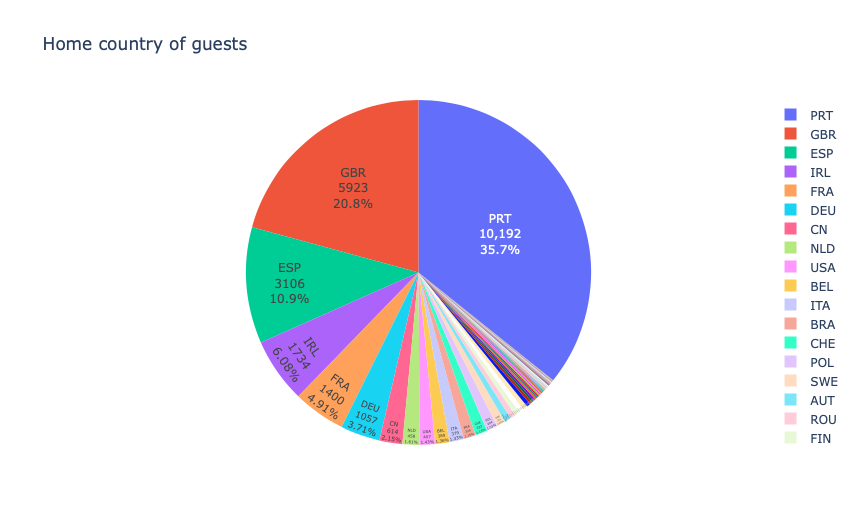
\includegraphics[width=0.8\linewidth]{images/Country_Percentage.png}
\end{center}
   \caption{The Percentage of Customer Origin Country}
\label{fig:CountryPercent}
\end{figure}

\begin{figure}[ht]
\begin{center}
    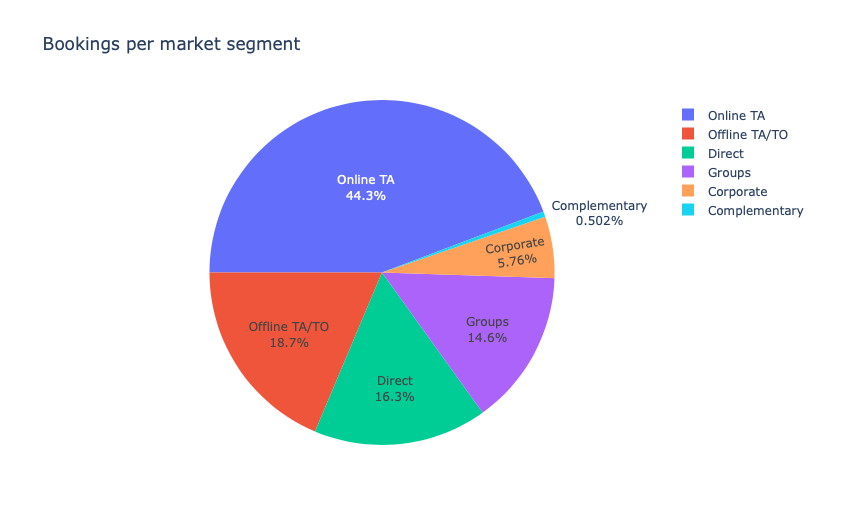
\includegraphics[width=0.8\linewidth]{images/Market_Percentage.png}
\end{center}
   \caption{The Percentage of Customer Market Segment}
\label{fig:MarketPercent}
\end{figure}


Overall, as showed in Figure~\ref{fig:ResortHotel}, the variables like \emph{Adults}, \emph{Children}, \emph{StaysInWeekendNights}, \emph{StaysInWeekNights}, \emph{Meal}, \emph{Country} and \emph{AssignedRoomType} are clearly distributed differently corresponding to the status of \emph{IsCanceled}. 

\begin{figure*}
\begin{center}
    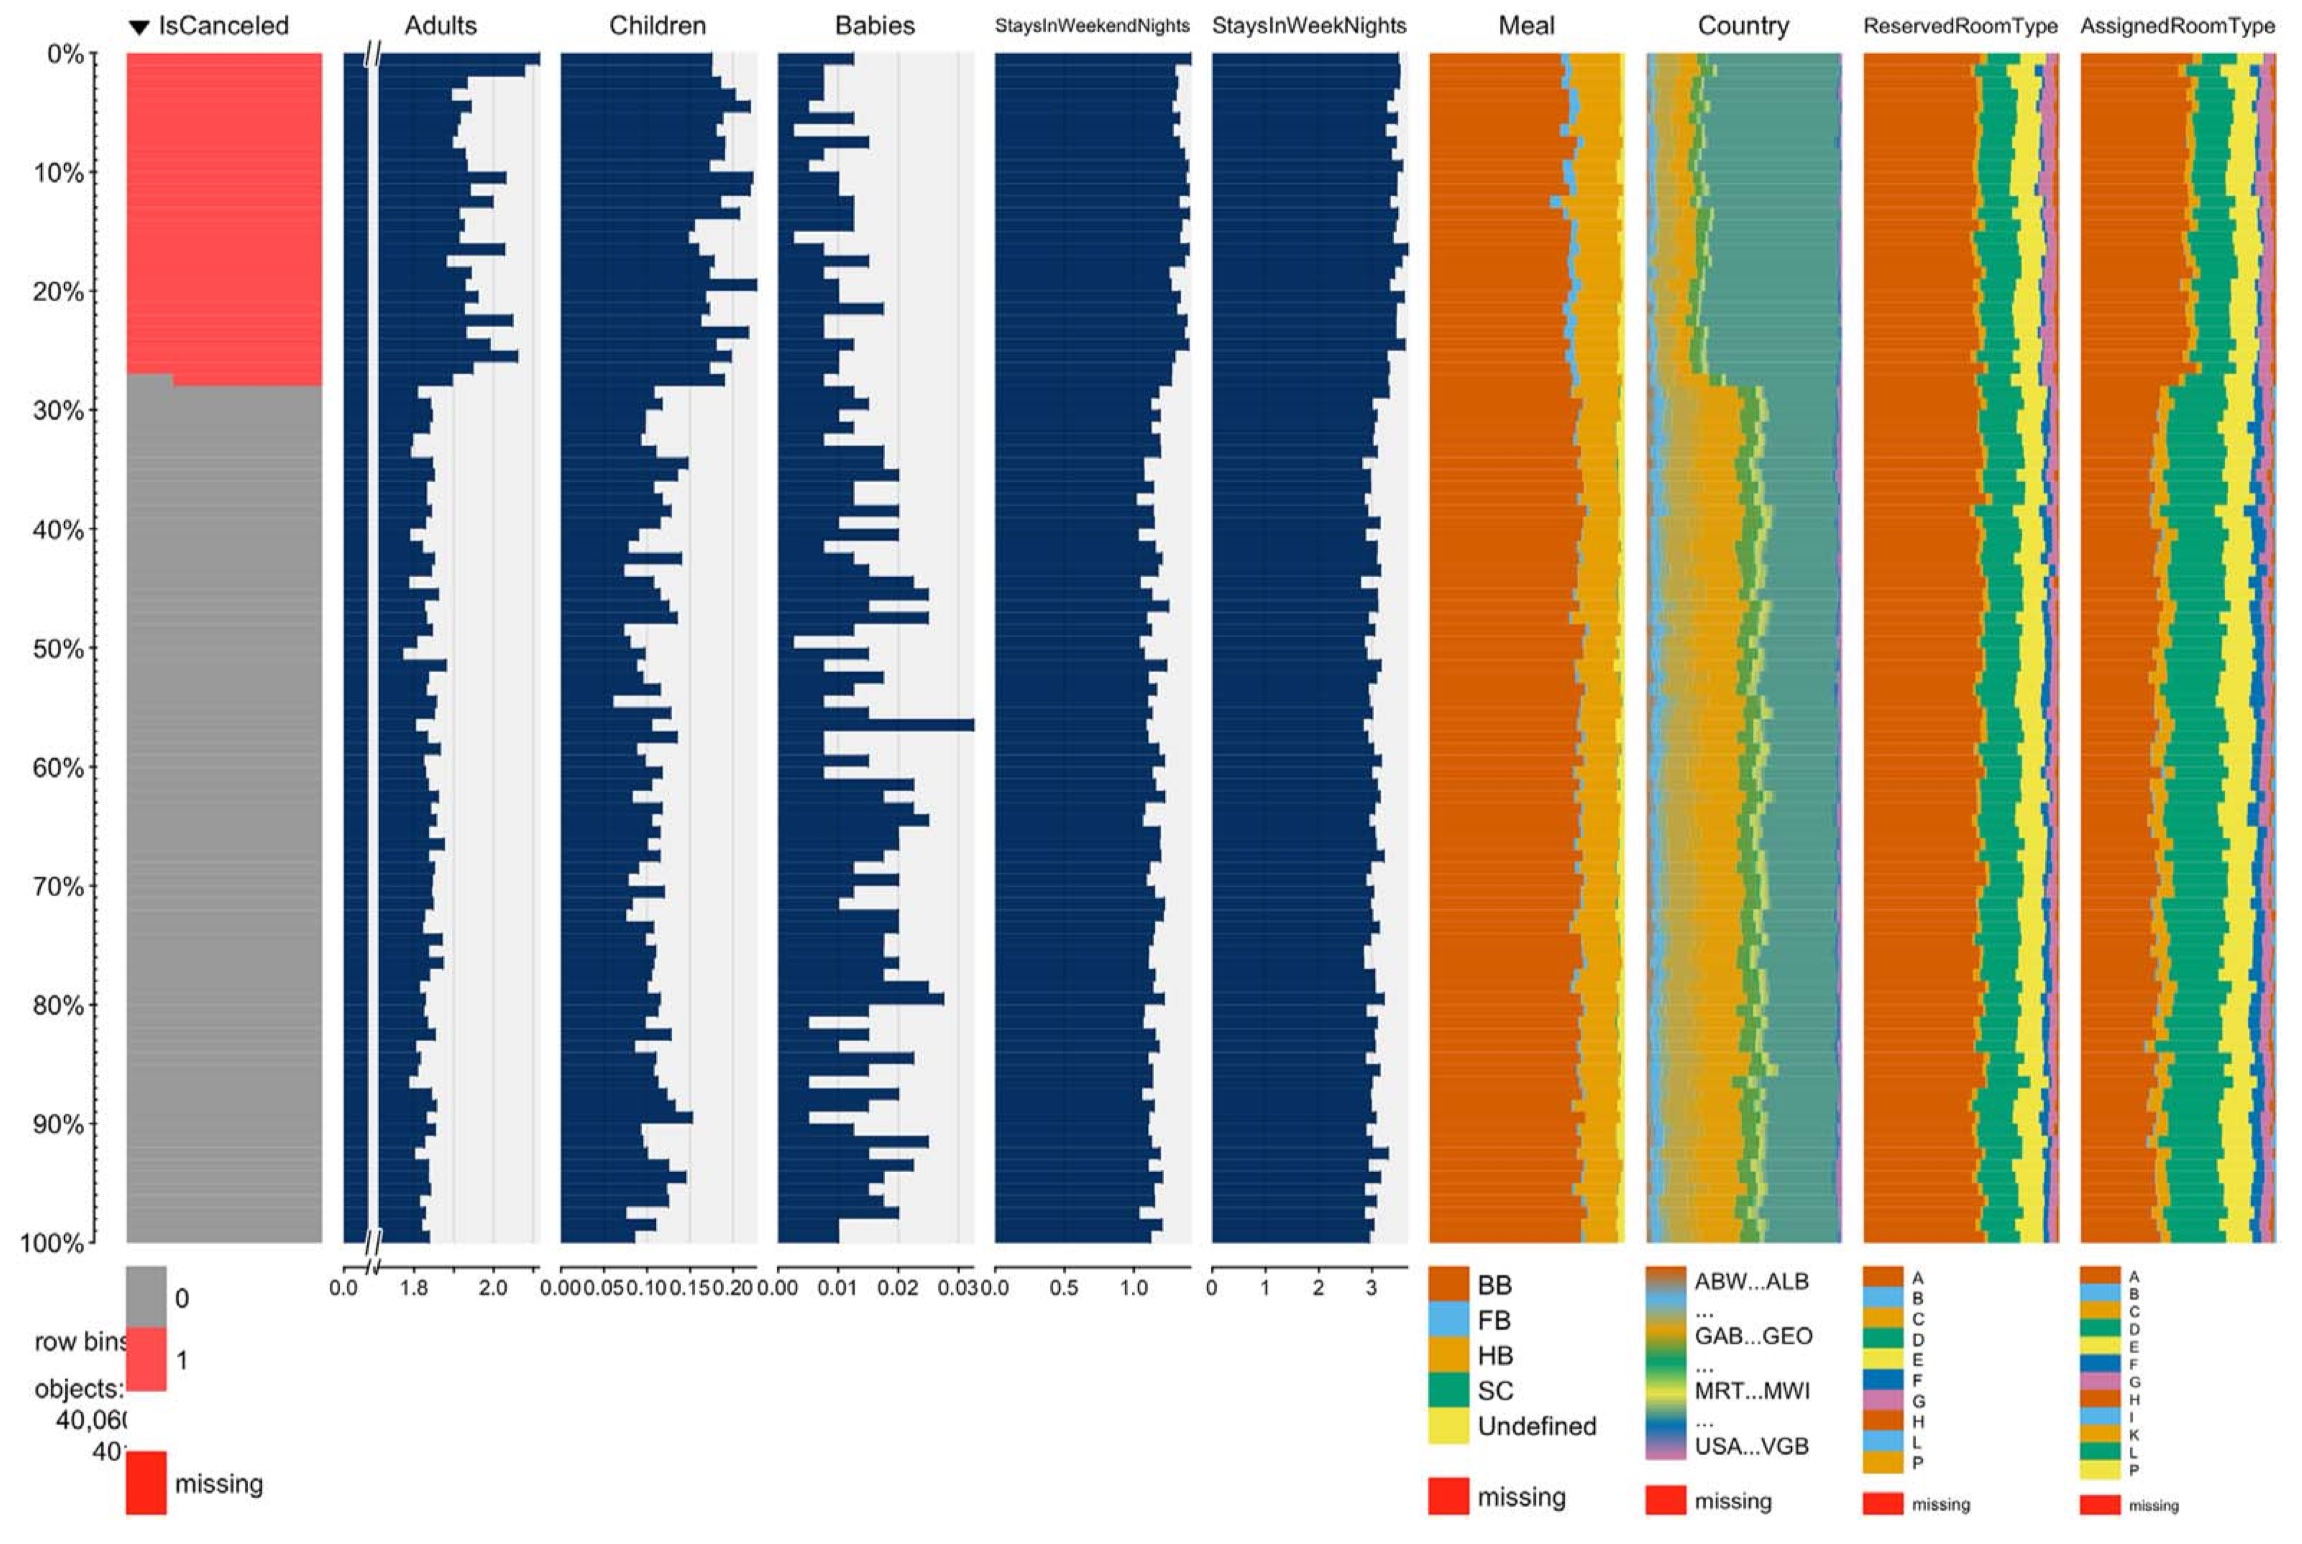
\includegraphics[width=0.8\linewidth]{images/Dataset_Resort_Hotel_Visualize.jpg}
\end{center}
   \caption{Dataset Visualization of All Observations}
\label{fig:ResortHotel}
\end{figure*}


%-------------------------------------------------------------------------
\subsection{Pre-Processing and Feature Engineering}


%-------------------------------------------------------------------------
\subsubsection{Data Imputation}
In our dataset, we have three features with null values showed in Table~\ref{Tab:NullDist}.
\begin{table}[ht]
\begin{center}
\begin{tabular}{|c|c|c|} \hline
    Feature & Number of Null & Percentage of Null\\ \hline
    \emph{Country} & 464 & 1.16\% \\ 
    \emph{Agent} & 8209 & 20.49\% \\ 
    \emph{Company} & 36952 & 92.24\% \\ \hline
\end{tabular}
\end{center}
\caption{\label{Tab:NullDist} Distribution of Null}
\end{table}

Because the null values in each feature stand for similar meaning, there is no need for regression in data imputation. We would just replace the nulls with particular integer or text instead.

For \emph{Country}, the null values means that the booking either not having country information so we replace the null values with "other" .

The null values in \emph{Agent} imply that the booking does not come from a booking agent. Similar for \emph{Company}, this feature implicate the ID of the company/entity that made the booking, and null value means that this is an individual booking. The data type for both \emph{Agent} and \emph{Company} is float, so we replaced the null values with $0$~\cite{ANTONIO201941}.

%-------------------------------------------------------------------------
\subsubsection{Category Numericalization}

Table~\ref{tab:DataTypes} describes the data type for each feature. To numericalize the categorical feature, we use different approaches:

\begin{itemize}
    \item Label Encoder: For \emph{ArrivalDateMonth}, which is originally month in text, we replace it by the numerical expression of month via label encoder. 
    \item Timestampe: The \emph{ReservationStatusDate} feature is originally object in format of "yyyy-mm-dd" and we reconstruct it into two numerical features: \emph{DayOfWeek} and \emph{DayOfYear} due to the seasonal nature of hotel demand.
    \item One-Hot Encoder: For other categorical variables, we simply resort to one-hot encoding.
\end{itemize}

% After the numericalization, the feature size becomes 192.


%-------------------------------------------------------------------------
\subsubsection{Feature Selection}
For our project, we are trying to prediction the cancellation status of a booking. After accessing the data, we found that \emph{IsCanceled} and \emph{ReservationStatus} are completely correlated with each other. When cancellation status is $0$ then reservation status would be \emph{CheckOut} otherwise cancellation status would be $1$. The feature importance generated by decision tree in Figure~\ref{fig:ResverationStatus} proves our guess. As only one prediction variable is needed, we decide to drop \emph{ReservationStatus} feature and use \emph{IsCanceled} as a binary label target. 

\begin{figure}[ht]
\begin{center}
    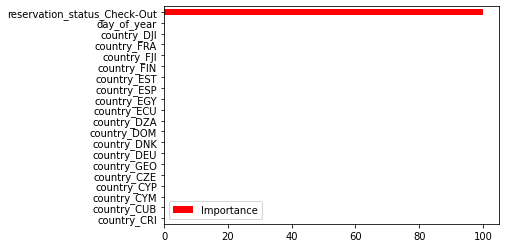
\includegraphics[width=0.8\linewidth]{images/Reservation_Status_Feature.png}
\end{center}
   \caption{The Importance of Reservation Status}
\label{fig:ResverationStatus}
\end{figure}


%-------------------------------------------------------------------------
\subsubsection{Feature Extraction}
To enhance the feature description and richness, based on the domain knowledge, three new features are created: 

\begin{itemize}
    \item \emph{IsFamily}: An binary indicator describing whether the hotel guests come as a family or not. 
        \begin{align*}
            \text {\emph{IsFamily}}=\left\{\begin{array}{ll}
            1 & \text{ if \emph{Adults} }>0 \text{ and } \\
              & {[\text{ \emph{Children} }>0 \text{ or } \text{ \emph{Babies} }>0]} \\
            0 & \text{ Otherwise }
            \end{array}\right.
        \end{align*}
    \item \emph{CustomerNumber}: The total number of customer.
        \begin{equation*}
            \emph{CustomerNumber} = \emph{Adults} + \emph{Children} + \emph{Babies}
        \end{equation*}
    \item \emph{NightNumber}: The total number of stayin nights.
        \begin{equation*} \begin{split}
            \emph{NightNumber} &= \emph{StaysInWeekendNights} \\
                &+ \emph{StaysInWeekNights} 
        \end{split} \end{equation*}
\end{itemize}

% Now the ultimate feature size is 195.


%-------------------------------------------------------------------------
\section{Problem Formulation}

The feature set are processed as above by a bunch of different encoding and extraction methods. As a result, we have 195 number-only features which are convenient for model deployment and friendly for description.

Our goal is to apply different machine learning techniques to predict whether a booking of 40,060 would be canceled or not based on the selected feature set and analyze the importance of each feature in that prediction (See Table \ref{tab:ProblemDef}).

\begin{table}[ht]
\begin{center}
\begin{tabular}{|c|c|} \hline
    $\mathbf{y}$ & $\mathbf{X}$ \\ \hline
    \emph{IsCanceled} & 194 Processed Features \\
\hline
\end{tabular}
\end{center}
\caption{\label{tab:ProblemDef} Statistically-Defined Problem}
\end{table}

%-------------------------------------------------------------------------
% \subsection{Loss Function}
Since this is a binary classification problem, where the canceled status $y=1$ denotes \emph{IsCanceled} while $y=0$ denotes \emph{IsNotCanceled}, then for the cancellation prediction, we use the cross-entropy loss function 
$$ \mathcal{L} = - [ y \log (p)  + (1-y) \log (1-p) ] $$
where $p$ is the predicted probability generated by the corresponding rank of $\mathbf{X}$.

The models we're going to explore in the next section are from the classic classification models such as logistic regression and decision trees and also some paper-based advanced models such as ensemble and DeepFM.


%-------------------------------------------------------------------------
\section{Methodologies}


\subsection{Logistic Regression (Baseline)}
The baseline model is set as the benchmark for the performance comparison. Since this is a binary classification problem and logistic regression can map all data points into a value between 0 and 1 by the sigmoid function, then it's used as the baseline model. 

Package: \href{https://scikit-learn.org/stable/modules/generated/sklearn.linear_model.LogisticRegression.html}{sklearn.linear\_model.LogisticRegression}


% \subsection{Time Series (Baseline?)} 
% Due to the nature of time sensitivity, hotel revenue management has resorted to time series to predict the demand for decades~\cite{weatherford2003comparison}. Here we use the vanilla time series model as baseline. TBC.

\subsection{Decision Tree}
The decision tree can break down the problem like binary classification into a bunch of subsets with homogeneous values. The splitting procedure is helpful to show the importance of each feature and thus provide us some insights. Afterall, a big advantage of decision tree is its interpretability which is close to human-being's decision-making process.

Package: \href{https://scikit-learn.org/stable/modules/generated/sklearn.tree.DecisionTreeClassifier.html}{sklearn.tree.DecisionTreeClassifier}

\subsection{Random Forest}
Random forest is an ensemble learning method which can be used for classification. It's comprised by a multitude of decision trees but without the cost of the overfitting prone and thus may have higher accuracy than decision tree.

Package: \href{https://scikit-learn.org/stable/modules/generated/sklearn.ensemble.RandomForestClassifier.html}{sklearn.ensemble.RandomForestClassifier}

\subsection{Extra Trees}
Extra trees is also ensembled by decision trees. However, different from random forests's subsampling and optimal splitting points, extra trees uses the whole original sample and split nodes by random. In other words, extra trees has a higher degree of randomness but also keeps optimization. Therefore, extra trees may executes faster~\cite{geurts2006}.

Package: \href{https://scikit-learn.org/stable/modules/generated/sklearn.ensemble.ExtraTreesClassifier.html}{sklearn.ensemble.ExtraTreesClassifier}

\subsection{Support Vector Machine}
Support vector machine is a good general-purpose classification algorithm. It aims to find the beset decision boundary that splits a dataset into two or more classes by maximum margin. Despite the disadvantage of the $\mathcal{O}(n^2 p)$ complexity, it's still feasible in our problem given the relatively small scale of dataset. 

Package: \href{https://scikit-learn.org/stable/modules/generated/sklearn.svm.SVC.html}{sklearn.svm.SVC}


\subsection{Neural Network}
The neural network, stems from the biological neurons mimic, is useful in classification domain. The key of neural network is the extraction of the linear combination of the features, and then models the observation as a nonlinear function of the fitted features. Therefore, the neural network can be used as a multi-step regression. Further, by increasing the hidden layers, we can construct a deep learning model to dissect the features and solve the binary classification problems to a fairly high degree.

Package: \href{https://scikit-learn.org/stable/modules/generated/sklearn.neural_network.MLPClassifier.html}{sklearn.neural\_network.MLPClassifier}


\subsection{XGBoost}
XGBoost is an algorithm designed by Dr. Tianqi Chen that is considered one of the fastest implementation of gradient tree boosting. It it suitable for medium and small structure data and can perform parallel processing to increase speed. By pruning and regularization, the model also outperform other boosting models in preventing over-fit. 

Package: \href{https://xgboost.readthedocs.io/en/latest/python/python_intro.html}{xgboost.XGBClassifier}


\subsection{AdaBoost}
AdaBoost is a meta-learning method that is initially created to increase the efficiency of binary classifiers and thus perfectly suits this problem~\cite{freund1999short}. The adaptive behavior allows it to focus on the mistake of weak classifier and then turn them into stronger ones. As a result, it can seize the depth of detail thoroughly.

Package: \href{https://scikit-learn.org/stable/modules/generated/sklearn.ensemble.AdaBoostClassifier.html}{sklearn.ensemble.AdaBoostClassifier}


\subsection{Soft-Voting (Ensemble)}
Soft voting is selected as our ultimate ensemble method. Whereas hard voting prefers a majority-take-all policy, soft voting can make use of each model more evenly by taking into account how certain each voter. In detail, after running the models above once, we can pick the most accurate ones to combine as a new multi-classifier estimator, where the voting weights are subject to the rank of accuracy.

Package: \href{https://scikit-learn.org/stable/modules/generated/sklearn.ensemble.VotingClassifier.html}{sklearn.ensemble.VotingClassifier}


\subsection{Deep Factorization-Machine}
DeepFM is a neural network framework that combines the power of factorization machines (FM) for recommendation and deep learning for feature learning in a new neural network architecture (DNN). It focuses on both the wide and deep. In the DeepFM's neural network part, the activation function of the hidden layer uses ReLu and tanh for non-linear signal mapping, and the sigmoid function is used as the output function for Click Through Rate (CTR) estimation.

FM is to extract the high-order features and solve the combination of features given the systematic coefficient. Due to the application of hidden variable, FM can stay a good performance even if under the circumstance of hidden variable. The DNN is to extract the low-order features. They shared a weight matrix, that is, embedding layor. DeepFM can build a model based on the interaction of high-order features and low-order features without feature engineering~\cite{guo2017deepfm}. The computation is showed as below.

$$ \hat{y}=\operatorname{sigmoid}\left(y_{FM}+y_{DNN}\right) $$

Since CTR is a variant of binary classification problem, and a deep learning network can solve the sparse feature dimension explosion, such as the feature \emph{Country} in our dataset, caused by one-hot encoding, then DeepFM is suitable for this problem.

Package: \href{https://deepctr-doc.readthedocs.io/en/latest/deepctr.models.deepfm.html}{deepctr.models.deepfm} and also self-construct via pytorch

\begin{figure}[ht]
\begin{center}
    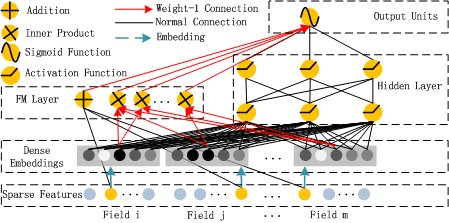
\includegraphics[width=0.8\linewidth]{images/DeepFM_Architecture.png}
\end{center}
   \caption{Wide and Deep Architecture of DeepFM}
\label{fig:DeepFM}
\end{figure}


\subsection{Others}

We tried several other methods such as Naive Bayes Gaussian but they perform awfully in this problem and thus are omitted here.


%-------------------------------------------------------------------------
\section{Experiments and Results}

%-------------------------------------------------------------------------
\subsection{Dataset Rebalance}
Imbalance can cause the underrepresention of the minority and thus harm the accuracy. By Figure~\ref{fig:ResortHotel}, the percentage of \emph{IsNotCanceled} is about 30\%, indicating slightly imbalance. The most traditional approaches to offset this impact is by resample, that is, undersample or oversample. However, both of them would bring new problems and a possible superior alternative is SMOTE. Their descriptions are as below.

\begin{itemize}
    \item Undersample: rebalancing the dataset by duplicating the minority class at the cost of overfitting
    \item Oversample: rebalancing the dataset by removing the majority class at the cost of information loss
    \item SMOTE: rebalancing the dataset by synthesizing new class from the minority ones with the aid of KNN and thus avoid the costs above
\end{itemize}

We test these three techniques by the prediction accuracy of the logistic regression baseline model given the balanced training set (Table~\ref{tab:RebalanceAcc}). All the rebalance methods successfully improve the prediction accuracy and among them, SMOTE's balanced dataset has the highest accuracy as expected. Therefore, we rebalance our training set by SMOTE before testing our models.

\begin{table}[ht]
\begin{center}
\begin{tabular}{|c|c|c|} \hline
Rebalance Method &  Balanced &  Imbalanced \\ \hline
SMOTE       &  0.8401 &  \\
Oversample  &  0.8387 & 0.8028 \\
Undersample &  0.8379 &  \\ \hline
\end{tabular}
\end{center}
\caption{\label{tab:RebalanceAcc} Dataset Rebalance Accuracy}
\end{table}


%-------------------------------------------------------------------------
\subsection{Metric}

To evaluate the performance of each model, we're going to generate the ROC curve plot to visualize the differences with the help of AUC scores. Due to the requirement of the precise cancellation prediction in hospitality to optimize the over-booking strategy, the prediction accuracy of each model has the last say of the performance. Also, runtime would also be taken into account since the deployment speed is important especially in the industry.

%-------------------------------------------------------------------------
\subsection{Hyperparameter Tuning}
Before deploying the models and comparing the results, we should first find the optimal hayperparameter combinations of the models. Here, we try to tune partial models which are easy to overfit and the hyperparameter has great impact. 


\subsubsection{Random Forest}
Since it's well-known that random forest can offer good performance with its default settings so this algorithm is less tunable~\cite{Probst_2019}. Therefore, We're going to pick just several parameters to see the difference. Because the number of trees is no risky to cause overfitting thus it should be set as large as possible~\cite{probst2017tune}. The grid search is showed below where the optimal parameters are bolder.

\begin{itemize}
    \item max\_features: auto, \textbf{sqrt}, log2
    \item min\_samples\_split: \textbf{2}, 5, 10
    \item n\_estimators: 100, 200, \textbf{500}
\end{itemize}


\subsubsection{Support Vector Machine}
Since in SVM, the overfit can be avoided by choosing appreciate kernel function and necessary regularization. It's important that we do tuning here to find the best pair of kernel and penalty. Hence, we decide to loop each kernel function plus a set of regularization parameter to see the best combination. The grid search is showed below where the optimal parameters are bolder, with an accuracy heatmap Figure~\ref{fig:SVMHeatmap}.

\begin{itemize}
    \item Kernel: \textbf{linear}, poly, rbf, sigmoid
    \item C (Regularization Parameter): 50, 10, 1.0, \textbf{0.1}, 0.01
\end{itemize}

\begin{figure}[ht]
\begin{center}
    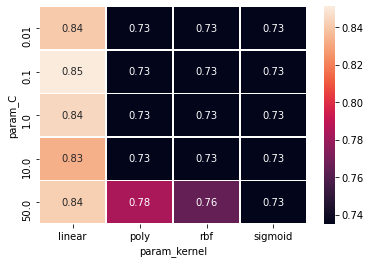
\includegraphics[width=0.8\linewidth]{images/SVM_Heatmap.png}
\end{center}
   \caption{Accuracy Heatmap of SVM Tuning}
\label{fig:SVMHeatmap}
\end{figure}


\subsubsection{Neural Network}
The activation functioins are for nonlinearity creation which invloves the deep learning models later, where both logsitic and ReLu are classical. The hidden layer size determines the complexity of model and thus a larger size may improves the accuracy. The grid search is showed below where the optimal parameters are bolder.

\begin{itemize}
    \item alpha: 1, 0.1, 0.01, \textbf{0.001}
    \item hidden\_layer\_sizes: (50, 50, 50), \textbf{(100, 100)}
    \item solver: \textbf{adam}, sgd
    \item activation: \textbf{logistic}, relu
\end{itemize}


%-------------------------------------------------------------------------
\subsection{Basic Model Implementation}
Due to the time limitation, it's not possible to tune all the models. However, we can pick the hyperparameter candidates as suitable as possible by the prior knowledge of other binary classification problems samples. Also, the tuned parameters above give us some insights. For instance, we set the n\_estimators as 500 in other tree family algorithms too due to their similarity with random forest.

During the empirical study, some models need a special handling of the training set and/or test set. For instance, as a gradient descend based algorithm, neural networks prefers the training set to be normally distributed data as a Gaussian with 0 mean and unit variance and thus a standardization is necessary. Another example is XGBoost, which requires the column number of training set and test set is the same. Hence, when deploying it to the balanced training set, we rebalance the test set as well.
 
By training each model excepts soft-voting and DeepFM and make a prediction on the test set, we generate an overlapped ROC curve with the AUC score of each model (Figure~\ref{fig:CompareROC}) for better visual comparison. Besides, we measure the execution time displayed as histogram in Figure~\ref{fig:Runtime}. A summary metric table is showed in Table~\ref{tab:ModelPerformance} which is comprised of the AUC score, accuracy score and runtime of each model, grouped by the imbalanced and balanced dataset. We will discuss it in the next section from different perspectives.

\begin{figure*}[h]
\begin{center}
    \centering
    \subfloat[\centering Imbalanced]{{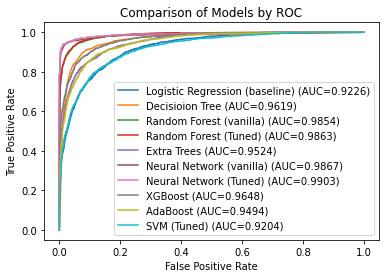
\includegraphics[width=7cm]{images/ROC_Imbalanced.png} }}%
    \qquad \qquad
    \subfloat[\centering Balanced]{{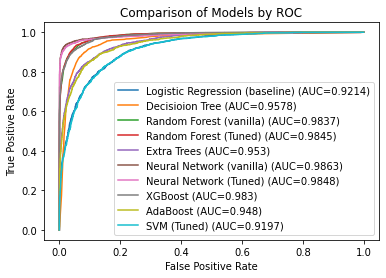
\includegraphics[width=7cm]{images/ROC_Balanced.png} }}%
\end{center}
    \caption{Basic Models Comparison by ROC}%
\label{fig:CompareROC}
\end{figure*}

\begin{table*}[h]
\begin{center}
\begin{tabular}{|c|c|c|c|c|c|c|} \hline
Model & AUC &  AUC* & Accuracy & Accuracy* & Runtime(s) & Runtime(s)* \\ \hline
Neural Network (Tuned)         
&  0.9885 &  0.9889 &    0.9725 &      0.9672 &    209.7754 &      253.2274 \\
Neural Network (vanilla)       
&  0.9868 &  0.9833 &    0.9705 &      0.9614 &    132.9359 &      125.3403 \\
Random Forest (Tuned)          
&  0.9863 &  0.9848 &    0.9467 &      0.9441 &     32.1794 &       54.7000 \\
Random Forest (vanilla)       
&  0.9853 &  0.9839 &    0.9458 &      0.9447 &      6.3899 &       11.2010 \\
Decision Tree                
&  0.9619 &  0.9555 &    0.9217 &      0.9146 &      0.5261 &        1.3537 \\
XGBoost                        
&  0.9648 &  0.9833 &    0.9096 &      0.9308 &     13.4476 &       20.0968 \\
AdaBoost                       
&  0.9494 &  0.9489 &    0.8938 &      0.8949 &     47.5919 &      102.2639 \\
Extra Trees                    
&  0.9527 &  0.9527 &    0.8812 &      0.8922 &     27.0275 &       44.5968 \\
SVM (Tuned)                    
&  0.9204 &  0.9199 &    0.8665 &      0.8326 &    989.7524 &     2564.1543 \\
Logistic Regression (baseline) 
&  0.9226 &  0.9218 &    0.8663 &      0.8361 &      7.4758 &        7.3667 \\ \hline
\end{tabular}
\end{center}
\caption{\label{tab:ModelPerformance} Basic Models Performance Comparison. Sorted in a descending order by the accuracy of imbalanced training, where the asterisk ($\star$) denotes being trained by balanced dataset.} 
\end{table*}

%-------------------------------------------------------------------------
\subsection{Advanced Exploration}

\subsubsection{Soft-Voting (Ensemble)}
After completing the basic models, we pick the top three models with the highest accuracy in balanced training set as showed in Table~\ref{tab:ModelPerformance}. Next, them are ensembled as a new estimator by soft-voting technique. The weight of their votes is descending based on the accuracy of the imbalanced training group. In this case, we combine tuned neural network, tuned random forest and decision tree with the weight ratio 2:2:1 because while tuned neural network has a very close accuracy as tuned random forest, decision tree has a relatively worse performance. The accuracy we got is 0.9752, higher than all the single classifiers we implemented so far.


\subsubsection{Deep Factorization-Machine}
We first use pytorch to construct a simply DeepFM network to test a subset with partial feature and the training loss per epochs is showed in Figure~\ref{fig:DeepFMLoss}. As the rise of training round, the parameters of model keep updating and therefore the loss value is decreasing. After about 40 rounds, the loss value remains nearly the same which indicts that the model begins to perform at the stable level and the efficiency of training is small after 40th round.

But since the DeepFM requires a special pre-processing of dataset to separate them as sparse and dense feature dictionaries, we resort to the deepctr package but unfortunately haven't completed it yet due to the time limitation and colab computing power constraint. Therefore, we cannot fully explore the potential of this state-of-the-art recommendation system algorithm and see whether it can be successfully transferred to another binary classification problem like the hotel demand.

\begin{figure}[H]
\begin{center}
    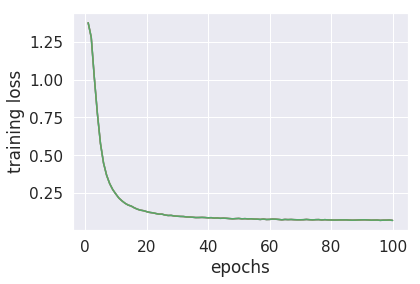
\includegraphics[width=0.8\linewidth]{images/DeepFM_Train_Loss.png}
\end{center}
   \caption{DeepFM: Training Loss vs Epochs}
\label{fig:DeepFMLoss}
\end{figure}

%-------------------------------------------------------------------------
\section{Conclusion and Discussion}


%-------------------------------------------------------------------------
\subsection{Feature Importance and Relationship}

With the help of decision tree, we get the feature importance (Figure~\ref{fig:FeatureImp}).

\begin{figure}[H]
\begin{center}
    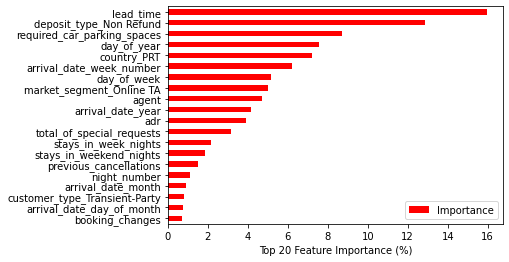
\includegraphics[width=0.8\linewidth]{images/Feature_Importance.png}
\end{center}
    \caption{Feature Importance}
\label{fig:FeatureImp}
\end{figure}

Although we cannot make an assertion of the causality from the feature importance, they provide us the pattern between the features and cancellation status. We will walk through a tip of them to guess the possible reasons behind. %Notes that all of their correlation is negative. 

\begin{enumerate}
    \item \emph{LeadTime}, the number of days that elapsed between the entering date of the booking into the PMS and the arrival date, is the most significant feature, with amost 15\% importance. It makes sense since the longer the duration before arrival, the larger the possibility that the guests may cancel the booking due to unexpected factors.
    \item The feature of the second importance is \emph{DepositType-NonRefund}, it's probably because the existance of refund could encourage the customers to cancel the booking without the cost of losing money.
    \item Next, \emph{RequiredCarParkingSpaces} is important. It is refer to the customers who are likely driving the car or plan to drive the car to the hotel. Their travels are more stable because they don't worry much about the weather condition and public traffic unlink the customers who go there by bus or plane. A group of them might already on the road when booking the hotel and thus less likely to cancel.
    \item The feature \emph{DayOfYear} is always important considering the seasonality of hospitality. It also shows that compared to other timestamps such as \emph{DayOfWeek}, \emph{DayOfMonth}, \emph{Month} and \emph{Year}, this feature has a much greater influence probably because the annual events such as holidays are more regular predictable. 
\end{enumerate}

Obviously, by the help of the important features we mentioned in graph and above, the hotel can predict the cancellation likelihood of a guest much easily. Moreover, the hotel can adjust the business strategy by these feature-based insights. For example, since the \emph{DayOfYear} is a significant indicator, the hotel can make their overbooking policy more aggressive during the off season to make the best use of their rooms. Also, when seeing a customer with a reuest of car parking spaces, the hotel should predict that this customer is very likely to show-up and can begin the welcome procedure more confidently.


%-------------------------------------------------------------------------
\subsection{Model Performance and Optimization}
As showed in ROC Comparison (Figure~\ref{fig:CompareROC}) and Accuracy Table (Table~\ref{tab:ModelPerformance}), nearly all the basic models we selected perform equal to or better than the performance of the logistic regression baseline. In the imbalacned training, the best ones without the vanilla are tuned neural network (0.9725), tuned random forest (0.9467) and decision tree (0.9619). 

A soft-voting ensemble estimator combined with these three classifiers has an outstanding accuracy 0.9752, outperforming any single of them. It shows the success that a proper comprehensive usage of models have the potential of exceeding the single classifier. This time we assigned the weight by ratio 2:2:1 by the scale of accuracy difference. However, this accuracy is only 0.0025 larger than the best single classifier, tuned neural network. In the future, the research can explore and compare different combination of the weight ratio to see whether weighting strictly based on the accuracy of single classifier is a good idea and whether a better ensemble can improve the accuracy significantly further.

The tuning technique grid search improves the accuracy but not that much. Both in neural network and random forest, we can see a trivial enhancement after tuning when being trained by the imbalanced dataset. However, they're worse than the vanilla ones in the balanced training. It's possible that because the vanilla we use here already has a reasonable default parameter based on the prior experience. It requires us to do a much larger set of hyperparameter combination further to justify this assertion when the time is allowed.

As showed in Figure~\ref{fig:Runtime}, the execution time of support vector machine is extremely high due to its $\mathcal{O}(n^2 p)$ complexity, whereas almost other models finish the implementation within 1-2 minutes. While SVM is suitable for classification, it needs some performance optimization when being deploying on the large size dataset.

\begin{figure}[ht]
\begin{center}
    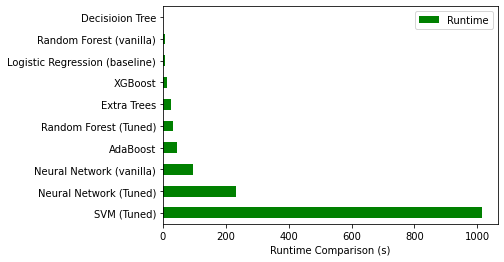
\includegraphics[width=0.8\linewidth]{images/Runtime.png}
\end{center}
   \caption{Runtime of Each Model}
\label{fig:Runtime}
\end{figure}

The difference between imbalanced and balanced dataset is subtle and it's not rare that the imbalanced one even has a higher accuracy than the balanced’s. Because rebalance reduces the possibility of overfitting, it makes sense that the classifier trained by balanced training set has lower prediction accuracy. % Probably by the same reason, the accuracy of the tuned models are worse than vanilla because while being exposed to a balanced dataset, the better model 

\newpage


%-------------------------------------------------------------------------
{\small
\bibliographystyle{ieee_fullname}
\bibliography{egbib}
}


%-------------------------------------------------------------------------
\section*{Acknowledgment}
The authors especially thank the University of Pennsylvania CIS520 Machine Learning instructors, Dr. Ungar and the TAs, for their advice and support throughout this project. We would also like to show our gratitude to Dr Antonio, Dr. Almeida and Dr. Nunes, who provide this dataset.

\end{document}
